\documentclass[12pt,fleqn]{article}\usepackage{../../common}
\begin{document}
Materyel Mekaniği - 2

Sonsuz Küçük (Infinitesimal) Gerilme Tensörü

Green gerilme tensörünü gördük, kuvvetli bir yaklaşım ama bizim daha çok
kullanacağımız şimdi anlatacağımız. Niye? Çünkü Green tensörü sonlu değişimler
için geçerli ama çoğu uygulamada bize lazım olan çok ufak yamulmalar. Ufak
değişimler derken, önceki dersteki (3) formülünden hareketle, oradaki en son
terimi hatırlarsak, çok ufak yamulmalar için $\nabla u^T \nabla u << \nabla u$
olur, yani ufak değişimlerde o karesel işlem $\nabla u$'dan daha ufak sonuç
verir. O zaman belli durumlarda son terim yaklaşık sıfır kabul edilebilir,
$\nabla u^T \nabla u \approx 0$. O zaman Green tensörü bu durumlarda yaklaşık
olarak alttaki gibi olur,

$$
\epsilon_{Green} \approx \frac{1}{2} (\nabla u + \nabla u^T )
$$

Bileşen formunda

$$
\epsilon_{ij} = \left(
\frac{\partial u_i}{\partial X_j} + \frac{\partial u_j}{\partial X_i}
\right)
$$

Bu tensör de simetrik, fakat sadece ufak şekil değişimleri, yamulmalar için
geçerli. Fakat zaten, mesela inşaat mühendisliği durumunda, binalar, demir
çubuklar (beam) ile iş yaptığımız zaman, bu tür şekil değişimi faraziyesi
yeterli. Çünkü eh, biraz düşünürsek eğer binamız büyük şekil değişimleri
yaşıyorsa önümüzde daha büyük bir problem var demektir.

Gerilme tensörü aslında bu konunun en zor bölümü denebilir; eğer öğrenciler bunu
anlarsa, konunun geri kalanı kolay olacak artık.

Cauchy Stres Tensörü

Gerilme tensöründen stres tensörlerine geldik. İlk önce çekiş (traction) ya da
stres vektöründen bahsedeceğiz. Diyelim ki elimizde bir çubuk var, onu ortadan
kestiğimizi düşünelim, ve iki parça ortaya çıkıyor. Şimdi belki lisans seviyesi
Statik dersinden hatırlayanlar olabilir, bir nesneyi (sanal olarak) kesince onun
iç kuvvetlerini serbest bırakmış oluyoruz. 

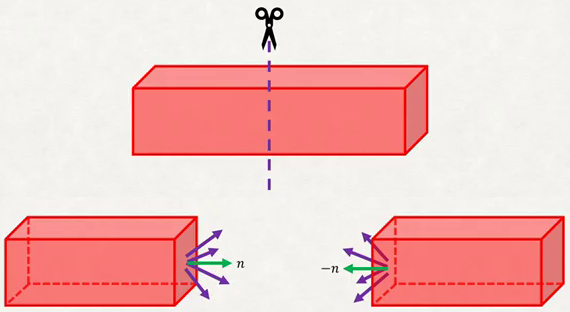
\includegraphics[width=20em]{phy_020_strs_02_01.png}

Kesit düzleminden bahsedelim önce, kesit tam dik olabilir ama bu şart değil,
nasıl olursa olsun o düzleme dik olan bir $\vec{n}$ vektörü ile bu kesitin
duruşunu temsil edebiliriz. 

Bu serbest bırakılmış iç kuvvetler darmadağın gözüküyor. Bir $\Delta A$
alanı tanımlayıp o alandaki tüm kuvvetleri alıp toplarsak bir $\Delta F$
elde edebiliriz, bu tek vektör daha derli toplu.

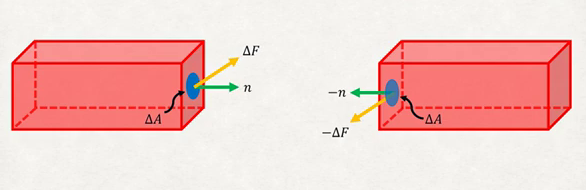
\includegraphics[width=20em]{phy_020_strs_02_02.png}

$\vec{n}$ ile tanımlı bir nokta etrafındaki düzlemin çekiş vektörünü (yani bir
noktadaki stres vektörü) şimdi şöyle tanımlıyoruz,

$$
t_n = \lim_{\Delta A \to 0} \frac{\Delta F}{\Delta A}
$$

Newton'un hareket kanunu üzerinden tabii ki sol taraftaki çekiş ile sağ
taraftaki birbirini dengelemeli, $t_n = -t_{-n}$.

Çekiş vektörü için formel tanım böyle. Ama kimse formel tanımı pek sevmiyor
sözel şekilde anlatırsak, çubuğu aldım ve kestim, Statik dersi der ki kaykılma
(shear), normal kuvvet ve eğilme momentimi böylece elde ederim. Bu üç boyutlu
nesnelerde olan şudur, çubuğu kesiyorum ve bileşenleri stres öğeleri olan tek
bir vektör elde ediyorum.

Şimdi çekiş vektörü kavramını daha basitleştirmeye uğraşalım. Bunun için
patatesimize geri dönüyoruz. Patatesten üç boyutlu sonsuz küçük küp şeklinde bir
parça çıkarttığımızı düşünelim şimdi,

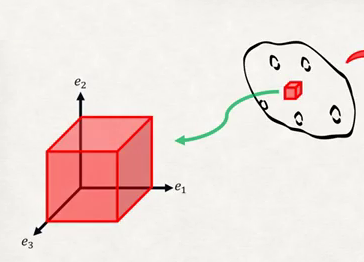
\includegraphics[width=15em]{phy_020_strs_02_03.png}

Bu ufak parça nesnenin bütünlüğünden çıkartıldığı için çekiş vektörlerinin
bu küpün yüzlerine etki eden stres vektörleri olduğunu söyleyebiliriz.

Küp sekli iyi bir seçim aslında çünkü her yüz kordinat eksendeki bir baz düzleme
paralel. Ayrıca $t_{e_1}$, $t_{e_2}$, $t_{e_3}$ yerine de daha iyi bir temsil
şekli bulabiliriz, küpün her yüzündeki bu $t$ çekiş vektörlerini de üç parçaya
ayırabiliriz,

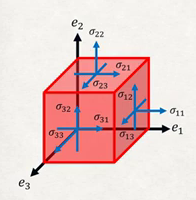
\includegraphics[width=10em]{phy_020_strs_02_04.png}

Bu şekildeki temsilin iyi bir tarafı her yüzdeki üç vektörün orijindeki
baz vektörlerle birebir uyuşması. O zaman mesela $t_{e_3}$'u o baz vektörlerin
lineer bir kombinasyonu olarak yazabilirim,

$$
t_{e_3} = \sigma_{31} e_1 + \sigma_{32} e_2 + \sigma_{33} e_3
$$

Üsttekini herhangi bir yüzey için yazarsak, yani $e_i$'in dik olduğu bir yüzey
için

$$
t_{e_i} = \sigma_{ij} e_j
$$

Einstein notasyonu kullandık, bu notasyonla her $i$ için mümkün tüm $j$'lerin üç
tane terimi ortaya çıkardığı kabul edilir.

Küpün yüzlerindeki çekiş vektörünü gösterebiliyoruz, fakat acaba herhangi bir
yöne bakan bir yüzey için stres vektörü ne olurdu? Bu ifadeyi genel bir şekilde
yazmak mümkün, hem bunu göstermek (ve ileride ispat etmek) için Cauchy Stres
Tetrahedon'u denen bir kurguyu anlatmamız lazım.

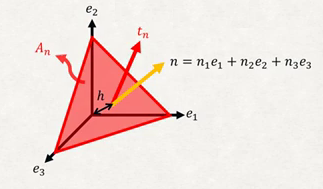
\includegraphics[width=20em]{phy_020_strs_02_05.png}

Tetrahedon ustteki gibi tanidik bir sekil. Cauchy Lemma'si ve Cauchy Kanununa
gore

$$
t_n = \sigma^T n
$$

olarak belirtilebilir, detaylı olarak belirtirsek,

$$
\left[\begin{array}{ccc}
t_{n1} \\ t_{n2} \\ t_{n3} 
\end{array}\right] =
\left[\begin{array}{ccc}
\sigma_{11} & \sigma_{21} & \sigma_{31} \\
\sigma_{12} & \sigma_{22} & \sigma_{32} \\
\sigma_{13} & \sigma_{23} & \sigma_{33} 
\end{array}\right]
\left[\begin{array}{ccc}
n_1 \\ n_2 \\ n_3
\end{array}\right]
$$

Bu formüldeki $\sigma$ Cauchy stres tensoru olarak adlandırılır. Üstteki ifade
şunu söylemiş oluyor aslında, üstünde kuvvet etkileri olan bir katı cisim bize
verilince yönden bağımsız bir Cauchy stres tensoru $\sigma$ elde edebiliriz,
yani öyle bir $\sigma$ vardır ki $n$ yönündeki $t_n$ elde etmek için
$t_n = \sigma^T n$ yapılabilir.

Cauchy tensorünün bazı özellikleri,

1) $\sigma$ simetriktir, yani $\sigma_{ij} = \sigma_{ji}$.

2) Öyle bir kordinat sistemi vardır ki bu sistemde $\sigma$ köşegendir. Lineer
cebirde köşegenleştirme vardır bildiğimiz gibi, burada o teknik uygulanır, bu
şekilde ana bileşen stresleri (principle stresses) denen stres vektörleri elde
edilebilir.

3) Feragat / teslim / esneme yüzeyi (yield surfaces) denen bir hesabı bu tensor
üzerinden yapmak mümkün. 






[devam edecek]

\end{document}
